\documentclass{article}
\usepackage{arxiv}

\usepackage[utf8]{inputenc}
\usepackage[english, russian]{babel}
\usepackage[T1]{fontenc}
\usepackage{url}
\usepackage{booktabs}
\usepackage{amsfonts}
\usepackage{nicefrac}
\usepackage{microtype}
\usepackage{lipsum}
\usepackage{graphicx}
\usepackage{natbib}
\usepackage{doi}
\usepackage{amsmath}
\DeclareMathOperator*{\argmax}{arg\,max}
\DeclareMathOperator*{\argmin}{arg\,min}


\title{Увеличение эффективности подбора гиперпараметров}

\author{ Валентин А. Абрамов \\
	Факультет вычислительной математики и кибернетики\\
	МГУ имени М. В. Ломоносова\\
	%% \AND
	%% Coauthor \\
	%% Affiliation \\
	%% Address \\
	%% \texttt{email} \\
	%% \And
	%% Coauthor \\
	%% Affiliation \\
	%% Address \\
	%% \texttt{email} \\
	%% \And
	%% Coauthor \\
	%% Affiliation \\
	%% Address \\
	%% \texttt{email} \\
}
\date{}

\renewcommand{\shorttitle}{\textit{arXiv} Template}

%%% Add PDF metadata to help others organize their library
%%% Once the PDF is generated, you can check the metadata with
%%% $ pdfinfo template.pdf
\hypersetup{
pdftitle={A template for the arxiv style},
pdfsubject={q-bio.NC, q-bio.QM},
pdfauthor={David S.~Hippocampus, Elias D.~Striatum},
pdfkeywords={First keyword, Second keyword, More},
}

\begin{document}
\maketitle

\begin{abstract}
Гиперпараметры являются важными параметрами алгоритмов машинного обучения, которые не могут быть определены в процессе обучения модели. Традиционные методы выбора гиперпараметров, такие как сеточный поиск или случайный поиск, могут быть неэффективными или требовать значительных вычислительных ресурсов, поэтому вместо них используют более сложные алгоритмы, например, эволюционные. Одним из таких алгоритмов является DEHB.

В данной статье предложено улучшение метода дифференциальной эволюции, лежащего в основе DEHB. Алгоритм DEHB жадный - постоянно переиспользует старые значения. Предложено добавлять шум во время мутации для увеличения покрытия пространства гиперпараметров.

Были представлены экспериментальные результаты, демонстрирующие эффективность этого метода в сравнении с базовым DEHB и традиционными методами выбора гиперпараметров. Результаты показывают, что изменение мутации может обеспечить более высокую точность модели при неизменном использовании вычислительных ресурсов.

\end{abstract}


\keywords{First keyword \and Second keyword \and More}

\section{Введение}

В последние годы машинное обучение стало одной из самых активно развивающихся областей в информационных технологиях. Чтобы достичь высокого качества моделей машинного обучения, необходимо правильно настроить гиперпараметры алгоритмов. Для каждой задачи значения параметров одной модели будут отличаться, и они могут сильно повлиять на целевую метрику. 
Гиперпараметрическая оптимизация - большая и перспективная область исследований. В статье \cite{bischl2021hyperparameter} приводится подробный обзор существующих методов, все алгоритмы формально описаны, поднимаются вопросы переобучения гиперпараметров на валидационную выборку и параллелизации алгоритмов. Для глубоких нейронных сетей также необходимо подбирать гиперпараметры, такие как число слоёв, learning rate и даже связи между слоями. О задачах гиперпараметрической оптимизации в нейронных сетях подробно написано в статье \cite{Talbi2020OptimizationOD}.

Задача автоматического подбора гиперпараметров активно исследуется. Ранее использовались методы перебора по сетке или случайного поиска значений, но эти методы имеют свои недостатки, такие как случайность, проклятие размерности, сложность подбора сетки, медленная скорость работы, невозможность учесть взаимосвязи между гиперпараметрами и зависимость целевой метрики от них. В 2011 году был создан подход SMBO - последовательная оптимизация, основанная на суррогатной функции (\cite{10.1007/978-3-642-25566-3_40}). В качестве суррогатной функции изначально брали гауссовские процессы, но они подходят не для всех задач, так как предназначены только для непрерывных гиперпараметров. Также был придуман алгоритм Succesive Halving (\cite{jamieson2015nonstochastic}), представляющий из себя жадный алгоритм, выделяющий больше ресурсов для оценки гиперпараметров с хорошим потенциалом.

На данный момент одним из лучших методов поиска является TPE (\cite{NIPS2011_86e8f7ab}), основанный на байесовском подходе. Также популярны методы, основанные на подходе SMBO, такие как SMAC, использующий случайный лес в качестве суррогата, или модели, использующие суррогат на основе гауссовских процессов. Лучше всего себя показывают методы, основанные на алгоритме Succesive Halving. На основе SH созданы алгоритмы HyperBand (\cite{li2018hyperband}), автоматически выделяющий ресурсы для нескольких запусков SH, BOHB (\cite{falkner2018bohb}), добавляющий в HyperBand суррогат на основе TPE и DEHB \cite{awad2021dehb}, добавляющий в HB идею дифференциальной эволюции. По текущим бенчмаркам DEHB является SOTA-алгоритмом подбора гиперпараметров.

В данный момент DEHB является одним из лучших алгоритмов, но у него есть недостатки. Из-за жадного переиспользования оптимальных значений при дифференциальной эволюции, модель застревает на плато в локальном минимуме. Чтобы этого избежать, предлагается добавлять шумовые векторы к мутантам при эволюции. Таким образом, благодаря шумовым векторам увеличится покрытие поверхности функции ошибки от гиперпараметров.

\section{Постановка задачи}
Задача гиперпараметрической оптимизации состоит в том, чтобы имея набор данных $X \in \mathbb{R}^{N\times d}, y \in \mathbb{R}^{N}$, пространство гиперпараметров $\Theta \in \mathbb{R}^k$, модель $f(\theta): \mathbb{R}^{d} \to \mathbb{R},\ \theta \in \Theta$, $f \in \mathbb{H}$ и целевую метрику $c(f, X, y): \mathbb{H} \times \mathbb{R}^{N\times d} \times \mathbb{R}^{N} \to \mathbb{R}$, найти $\theta^*$ такую, что выполнено
$$\theta^* = \argmin_{\theta} c(f(\theta), X, y)$$
Таким образом, зная модель $f$, пространство гиперпараметров $\Theta$, набор данных $X, y$ и целевую метрику $c$, необходимо найти набор гиперпараметров $\theta^*$, при котором целевая метрика $c$ наименьшая при обучении модели $f$ на данных $X, y$.
В нашей работе будет модифицирован метод подбора оптимальных гиперпараметров DEHB - Differential Evolution HyperBand. В нём  один раз сэмплируются кандидаты-наборы гиперпараметров из равномерного распределения, далее запускается процесс эволюции, в котором лучшие кандидаты передаются горизонтально в Succesive Halving сетках для одинаковых значений бюджета. Для мутации сэмплируются лучшие кандидаты из предыдущего значения бюджета в текущей SH сетке.

% \label{sec:headings}

% \lipsum[4] See Section \ref{sec:headings}.

% \subsection{Headings: second level}
% \lipsum[5]
% \begin{equation}
% 	\xi _{ij}(t)=P(x_{t}=i,x_{t+1}=j|y,v,w;\theta)= {\frac {\alpha _{i}(t)a^{w_t}_{ij}\beta _{j}(t+1)b^{v_{t+1}}_{j}(y_{t+1})}{\sum _{i=1}^{N} \sum _{j=1}^{N} \alpha _{i}(t)a^{w_t}_{ij}\beta _{j}(t+1)b^{v_{t+1}}_{j}(y_{t+1})}}
% \end{equation}

% \subsubsection{Headings: third level}
% \lipsum[6]

% \paragraph{Paragraph}
% \lipsum[7]



% \section{Examples of citations, figures, tables, references}
% \label{sec:others}

% \subsection{Citations}
% Citations use \verb+natbib+. The documentation may be found at
% \begin{center}
% 	\url{http://mirrors.ctan.org/macros/latex/contrib/natbib/natnotes.pdf}
% \end{center}

% Here is an example usage of the two main commands (\verb+citet+ and \verb+citep+): Some people thought a thing \citep{kour2014real, hadash2018estimate} but other people thought something else \citep{kour2014fast}. Many people have speculated that if we knew exactly why \citet{kour2014fast} thought this\dots

% \subsection{Figures}
% \lipsum[10]
% See Figure \ref{fig:fig1}. Here is how you add footnotes. \footnote{Sample of the first footnote.}
% \lipsum[11]

% \begin{figure}
% 	\centering
% 	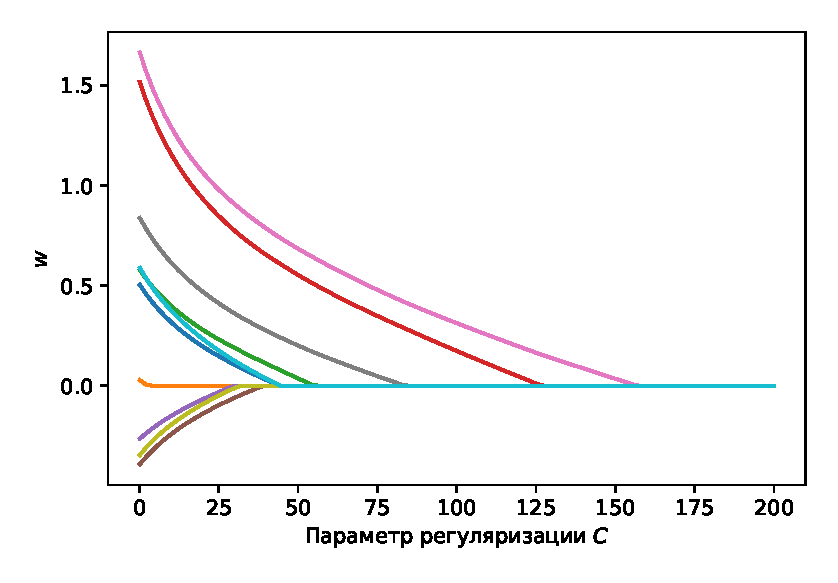
\includegraphics[width=0.5\textwidth]{../figures/log_reg_cs_exp.eps}
% 	\caption{Sample figure caption.}
% 	\label{fig:fig1}
% \end{figure}

% \subsection{Tables}
% See awesome Table~\ref{tab:table}.

% The documentation for \verb+booktabs+ (`Publication quality tables in LaTeX') is available from:
% \begin{center}
% 	\url{https://www.ctan.org/pkg/booktabs}
% \end{center}


% \begin{table}
% 	\caption{Sample table title}
% 	\centering
% 	\begin{tabular}{lll}
% 		\toprule
% 		\multicolumn{2}{c}{Part}                   \\
% 		\cmidrule(r){1-2}
% 		Name     & Description     & Size ($\mu$m) \\
% 		\midrule
% 		Dendrite & Input terminal  & $\sim$100     \\
% 		Axon     & Output terminal & $\sim$10      \\
% 		Soma     & Cell body       & up to $10^6$  \\
% 		\bottomrule
% 	\end{tabular}
% 	\label{tab:table}
% \end{table}

% \subsection{Lists}
% \begin{itemize}
% 	\item Lorem ipsum dolor sit amet
% 	\item consectetur adipiscing elit.
% 	\item Aliquam dignissim blandit est, in dictum tortor gravida eget. In ac rutrum magna.
% \end{itemize}


\bibliographystyle{unsrtnat}
\bibliography{references}

\end{document}
